\documentclass[a4paper,11pt]{article}

% Kodovani (cestiny) v dokumentu: utf-8
%\usepackage[cp1250]{inputenc}	% Omezena stredoevropska kodova stranka, pouze MSW.
\usepackage[utf8]{inputenc}	% Doporucujeme pouzivat UTF-8 (unicode).

\usepackage[margin=2cm]{geometry}
\newtoks\jmenopraktika \newtoks\jmeno \newtoks\datum
\newtoks\obor \newtoks\skupina \newtoks\rocnik \newtoks\semestr
\newtoks\cisloulohy \newtoks\jmenoulohy
\newtoks\tlak \newtoks\teplota \newtoks\vlhkost

\jmenopraktika={Fyzikální praktikum 1}
\jmeno={Lukáš Lejdar}
\datum={19 března 2024}
\obor={F}
\skupina={Út 16:00}

\cisloulohy={8}
\jmenoulohy={Měření teploty}

\tlak={101{,}35}
\teplota={21,1}
\vlhkost={47.7}


%%%%%%%%%%% Uzitecne balicky:
\usepackage[czech]{babel}
\addto\captionsczech{\renewcommand{\figurename}{Graf}}

\usepackage{graphicx}
\usepackage{amsmath}
\usepackage{xspace}
\usepackage{url}
\usepackage{indentfirst}
\usepackage{wrapfig}
\usepackage{xcolor}
\definecolor{bg}{HTML}{282828}

%%%%%% Zamezeni parchantu:
\widowpenalty 10000 \clubpenalty 10000 \displaywidowpenalty 10000
%%%%%% Parametry pro moznost vsazeni vetsiho poctu obrazku na stranku
\setcounter{topnumber}{3}	  % max. pocet floatu nahore (specifikace t)
\setcounter{bottomnumber}{3}	  % max. pocet floatu dole (specifikace b)
\setcounter{totalnumber}{6}	  % max. pocet floatu na strance celkem
\renewcommand\topfraction{0.9}	  % max podil stranky pro floaty nahore
\renewcommand\bottomfraction{0.9} % max podil stranky pro floaty dole
\renewcommand\textfraction{0.1}	  % min podil stranky, ktery musi obsahovat text
\intextsep=8mm \textfloatsep=8mm  %\intextsep pro ulozeni [h] floatu a \textfloatsep pro [b] or [t]

% Tecky za cisly sekci:
\renewcommand{\thesection}{\arabic{section}.}
\renewcommand{\thesubsection}{\thesection\arabic{subsection}.}
% Jednopismenna mezera mezi cislem a nazvem kapitoly:
\makeatletter \def\@seccntformat#1{\csname the#1\endcsname\hspace{1ex}} \makeatother
%
\newcommand{\vsn}[4]{\ensuremath{#1 =} #2(#3)\,#4}
\newcommand{\vrn}[6]{\ensuremath{#1 =} (#2 $\pm$ #3)\,#4 ($p=$ #5\,\%, $\nu=$ #6)}


%%%%%%%%%%%%%%%%%%%%%%%%%%%%%%%%%%%%%%%%%%%%%%%%%%%%%%%%%%%%%%%%%%%%%%%%%%%%%%%
% Zacatek dokumentu
%%%%%%%%%%%%%%%%%%%%%%%%%%%%%%%%%%%%%%%%%%%%%%%%%%%%%%%%%%%%%%%%%%%%%%%%%%%%%%%

\begin{document}

\thispagestyle{empty}

{
\begin{center}
\sf 
{\Large Ústav fyziky a technologií plazmatu Přírodovědecké fakulty Masarykovy univerzity} \\
\bigskip
{\huge \bfseries FYZIKÁLNÍ PRAKTIKUM} \\
\bigskip
{\Large \the\jmenopraktika}
\end{center}

\bigskip

\sf
\noindent
\setlength{\arrayrulewidth}{1pt}
\begin{tabular*}{\textwidth}{@{\extracolsep{\fill}} l l}
\large {\bfseries Zpracoval:}  \the\jmeno & \large  {\bfseries Naměřeno:} \the\datum\\[2mm]
\large  {\bfseries Obor:} \the\obor  \hspace{40mm}  {\bfseries Skupina:} \the\skupina %
&\large {\bfseries Testováno:}\\
\\
\hline
\end{tabular*}
}

\bigskip

{
\sf
\noindent \begin{tabular}{p{4cm} p{0.6\textwidth}}
\Large  Úloha č. {\bfseries \the\cisloulohy:} \par
\smallskip
$T=\the\teplota$~$^\circ$C \par
$p=\the\tlak$~kPa \par
$\varphi=\the\vlhkost$~\%
&\Large \bfseries \the\jmenoulohy  \\[2mm]
\end{tabular}
}

\vskip1cm

\section{Úkoly}

\subsection{Identifikace teplotních čidel, relaxační doba}

\begin{enumerate}
  \item V olejové lázni proměřte teplotní závislost elektrického odporu či napětí neznámých odporových a termoelektrických čidel. Teplotu nechte
vzrůstat v rozsahu 20 – 120 °C, závislosti zaznamenejte s krokem cca 5 °C. 

  \item Stanovte relaxační dobu vybraných čidel:
  \begin{enumerate}
  \item zapouzdřeného čidla (např. odporového čidla Pt 1000),
  \item nezapouzdřeného čidla (např. termoelektrického článku typu K).
  \end{enumerate}

\end{enumerate}

\subsection{Měření teploty infračerveným teploměrem}

\begin{enumerate}
\item Vyhřejte měděnou desku pokrytou černým, bílým a aluminiovým žáruvzdorným lakem na
plotýnkovém vařiči asi na teplotu asi 300 ◦C. Poté vařič vypněte. Nastavte na IR teploměru
emisivitu $\epsilon$ = 1. Z údaje IR teploměru získaného z lesklého a černého povrchu a skutečné
teploty desky měřené termočlánkem určete emisivity všech tří povrchů. 
\item Změřte teplotu černého povrchu zahřátého asi na 300◦C přes „okénko“ z různých materiálů. Porovnejte vždy teploty měřené pouze
infračerveným teploměrem s okénkem a bez okénka. Máme sadu „okének“, která zahrnuje
polykarbonát, sklo, SiO2, NaCl, CaF2 a KBr (dielektrika), Ge, Si a GaAs (polovodiče) a
Cu (kov). 
\item Změřte teplotu měděné plotny předem vychlazené v mrazničce pomocí kontaktního a IR
teploměru. Oběma teploměry proměřte a) povrch s námrazou, b) čistý kovový povrch, ze
kterého námrazu setřete žiletkou. Porovnejte údaje z obou teploměrů a spočtěte emisivitu
obou povrchů. Jakou „barvu“ má led?

\end{enumerate}

\subsection{Měření s můstkem}

\begin{enumerate}
  \item Vyzkoušejte míru kompenzace ohřevu odporového čidla při můstkovém zapojení dvojice
čidel. Umístěte obě čidla těsně k sobě, abychom mohli předpokládat stejnou teplotu bezprostředního okolí. Vyvažte
můstek, změřte si napájecí napětí při vyváženém můstku. Nechte protékat měřicí proud po
dobu asi 10 minut (mezitím plňte jiné úkoly). Pak jedno čidlo vložte do těsné polystyrénové
krabičky a opět vyčkejte asi 10 minut. Porovnejte a komentujte výsledky.
 
\end{enumerate}

\section{Postup měření}

\subsection{Odporová čidla, termočlánky a jeijch realaxační doba}

\begin{enumerate}
\item Odpor kovového vodiče s teplotou roste. Měřením odporu čidla tedy můžeme měřit teplotu. 
V úloze 1.1 se pokusíme zkalibrovat dvě taková čidala

\begin{equation}
R = R_0(1+\alpha \Delta t),
\end{equation}

kde $R_0$ je odpor čidla při některé referenční hodnotě a $\alpha$ teplotní odporový koeficient.  

\item Termočlánek je vyrobený spojem dvou různých matriálů. Pokud teplot spojů je různá, 
vznikne na termočlánku termoelektrické napětí, které je úměrné rozdílu teplot. Pokusíme se zkalibrovat i jeden termočlánek.

\begin{equation}
U=\beta\Delta t,
\end{equation}

kde $\beta$ je tzv. Seebeckův termoelektrický koeficient.
\end{enumerate}

Ve většině případů nejsou kladeny velké nároky na rychlost reakce teploměru. Přesto mohou být situace, kdy je
nutné měřit rychlé změny teploty – adiabatické expanze a komprese, silné exotermické reakce,
rychlá žíhání ohřevem laserovým nebo elektronovým svazkem apod.
Předpokládejme, že měřená teplota se změní skokem z hodnoty t1 na t2. Reakce čidla na změnu
teploty není okamžitá, ale probíhá s jistým zpožděním. Nejčastěji se předpokládá vztah

\begin{equation}
  t(\tau) = t_2 - (t_2-t_1)e^{\frac{\tau}{\tau_m}},
\end{equation}

, kde $\tau_m$ je relaxační doba. V druhé části úlohy jedna změříme relaxační dobu
jednoho zapouzdřeného odporového čidla a nezapouzdřeného termoelektrického článku typu K.

\subsection{Infračervené teploměry}

Podle Stefanova – Boltzmanova zákona platí, že intenzita elektromagnetického záření černého tělesa je úměrná čtvrté mocnině teploty tohoto tělesa.

\begin{equation}
  I_{\text{čt}} = \sigma T^4 
\end{equation}

Pro tělesa, které dokonale černá nejsou potom můžeme zavést emisivitu $\epsilon$ jako
odchylku vyzařování konkrétního povrchu od vyzařování dokonale černého tělesa.

\begin{equation}
  \epsilon = \frac{T_p^4}{T_{\text{čt}}^4}, \\
\end{equation}

kde v případě měření IR bude hodnota $T_p$ změřená teplota. a $T_{\text{čt}}$ zkutečná teplota tělesa. 
Se znalostí emisivity lze skutečnou teplotu spočíta. 
Pro zkoumání propustností různých materiálů použijeme upravený vztah,

\begin{equation}
\tau = \frac{T_0}{T_v}
\end{equation}

kde $T_0$ je hodnota naměřená IR teploměrem skrze daný matriál a $T_v$ je skutečná teplota tělesa.

\newpage

\subsection{Měření malých teplotních rozdílů}

Teplotní rozdíl můžeme samozřejmě vždy měřit i odečtením hodnot naměřených samostatnými teploměry. 
Takový postup, ale bývá pro velmi nepřesný. 
Rozdíly teplot v řádech podobných chybě samostatného teploměru ztratí veškerou přesnost původního měření.

V úloze použijeme Wheatstoneův můstek se dvěma odporovými čidli $R_1$ a $R_2$, konstruovaný právě na měření malých teplotních rozdílů.

\begin{figure}[ht]
  \centering
  \includegraphics[width=0.45\textwidth]{mustek_diagram.png}
  \caption{Wheatstoneův můstek se dvěma odporovými čidly $R_1$ a $R_2$}
\end{figure}

Pro praktické měření Wheatstonovým můstkem používáme approximativní vztah

\begin{equation}
\Delta t = \frac{4U}{U_0 \alpha}, \\
\end{equation}

kde $U_0$ je napájecí napětí a $\alpha$ teplotní koeficient odporu.

\newpage

\section{Výsledky měření}

\subsection{Kalibrace odporových čidel}

\begin{figure}[ht]
  \centering
  \include{olej_dif_cidlo.tex}
  \caption{}
\end{figure}

\begin{figure}[ht]
  \centering
  % GNUPLOT: LaTeX picture with Postscript
\begingroup
  \makeatletter
  \providecommand\color[2][]{%
    \GenericError{(gnuplot) \space\space\space\@spaces}{%
      Package color not loaded in conjunction with
      terminal option `colourtext'%
    }{See the gnuplot documentation for explanation.%
    }{Either use 'blacktext' in gnuplot or load the package
      color.sty in LaTeX.}%
    \renewcommand\color[2][]{}%
  }%
  \providecommand\includegraphics[2][]{%
    \GenericError{(gnuplot) \space\space\space\@spaces}{%
      Package graphicx or graphics not loaded%
    }{See the gnuplot documentation for explanation.%
    }{The gnuplot epslatex terminal needs graphicx.sty or graphics.sty.}%
    \renewcommand\includegraphics[2][]{}%
  }%
  \providecommand\rotatebox[2]{#2}%
  \@ifundefined{ifGPcolor}{%
    \newif\ifGPcolor
    \GPcolorfalse
  }{}%
  \@ifundefined{ifGPblacktext}{%
    \newif\ifGPblacktext
    \GPblacktexttrue
  }{}%
  % define a \g@addto@macro without @ in the name:
  \let\gplgaddtomacro\g@addto@macro
  % define empty templates for all commands taking text:
  \gdef\gplbacktext{}%
  \gdef\gplfronttext{}%
  \makeatother
  \ifGPblacktext
    % no textcolor at all
    \def\colorrgb#1{}%
    \def\colorgray#1{}%
  \else
    % gray or color?
    \ifGPcolor
      \def\colorrgb#1{\color[rgb]{#1}}%
      \def\colorgray#1{\color[gray]{#1}}%
      \expandafter\def\csname LTw\endcsname{\color{white}}%
      \expandafter\def\csname LTb\endcsname{\color{black}}%
      \expandafter\def\csname LTa\endcsname{\color{black}}%
      \expandafter\def\csname LT0\endcsname{\color[rgb]{1,0,0}}%
      \expandafter\def\csname LT1\endcsname{\color[rgb]{0,1,0}}%
      \expandafter\def\csname LT2\endcsname{\color[rgb]{0,0,1}}%
      \expandafter\def\csname LT3\endcsname{\color[rgb]{1,0,1}}%
      \expandafter\def\csname LT4\endcsname{\color[rgb]{0,1,1}}%
      \expandafter\def\csname LT5\endcsname{\color[rgb]{1,1,0}}%
      \expandafter\def\csname LT6\endcsname{\color[rgb]{0,0,0}}%
      \expandafter\def\csname LT7\endcsname{\color[rgb]{1,0.3,0}}%
      \expandafter\def\csname LT8\endcsname{\color[rgb]{0.5,0.5,0.5}}%
    \else
      % gray
      \def\colorrgb#1{\color{black}}%
      \def\colorgray#1{\color[gray]{#1}}%
      \expandafter\def\csname LTw\endcsname{\color{white}}%
      \expandafter\def\csname LTb\endcsname{\color{black}}%
      \expandafter\def\csname LTa\endcsname{\color{black}}%
      \expandafter\def\csname LT0\endcsname{\color{black}}%
      \expandafter\def\csname LT1\endcsname{\color{black}}%
      \expandafter\def\csname LT2\endcsname{\color{black}}%
      \expandafter\def\csname LT3\endcsname{\color{black}}%
      \expandafter\def\csname LT4\endcsname{\color{black}}%
      \expandafter\def\csname LT5\endcsname{\color{black}}%
      \expandafter\def\csname LT6\endcsname{\color{black}}%
      \expandafter\def\csname LT7\endcsname{\color{black}}%
      \expandafter\def\csname LT8\endcsname{\color{black}}%
    \fi
  \fi
    \setlength{\unitlength}{0.0500bp}%
    \ifx\gptboxheight\undefined%
      \newlength{\gptboxheight}%
      \newlength{\gptboxwidth}%
      \newsavebox{\gptboxtext}%
    \fi%
    \setlength{\fboxrule}{0.5pt}%
    \setlength{\fboxsep}{1pt}%
    \definecolor{tbcol}{rgb}{1,1,1}%
\begin{picture}(7920.00,5040.00)%
    \gplgaddtomacro\gplbacktext{%
      \csname LTb\endcsname%%
      \put(946,704){\makebox(0,0)[r]{\strut{}$1000$}}%
      \put(946,1161){\makebox(0,0)[r]{\strut{}$1100$}}%
      \put(946,1618){\makebox(0,0)[r]{\strut{}$1200$}}%
      \put(946,2076){\makebox(0,0)[r]{\strut{}$1300$}}%
      \put(946,2533){\makebox(0,0)[r]{\strut{}$1400$}}%
      \put(946,2990){\makebox(0,0)[r]{\strut{}$1500$}}%
      \put(946,3447){\makebox(0,0)[r]{\strut{}$1600$}}%
      \put(946,3905){\makebox(0,0)[r]{\strut{}$1700$}}%
      \put(946,4362){\makebox(0,0)[r]{\strut{}$1800$}}%
      \put(946,4819){\makebox(0,0)[r]{\strut{}$1900$}}%
      \put(1078,484){\makebox(0,0){\strut{}$20$}}%
      \put(2250,484){\makebox(0,0){\strut{}$40$}}%
      \put(3422,484){\makebox(0,0){\strut{}$60$}}%
      \put(4593,484){\makebox(0,0){\strut{}$80$}}%
      \put(5765,484){\makebox(0,0){\strut{}$100$}}%
      \put(6937,484){\makebox(0,0){\strut{}$120$}}%
    }%
    \gplgaddtomacro\gplfronttext{%
      \csname LTb\endcsname%%
      \put(209,2761){\rotatebox{-270.00}{\makebox(0,0){\strut{}Odpor [$\Omega$]}}}%
      \put(4300,154){\makebox(0,0){\strut{}teplota °C}}%
    }%
    \gplbacktext
    \put(0,0){\includegraphics[width={396.00bp},height={252.00bp}]{olej_odporova_cidla}}%
    \gplfronttext
  \end{picture}%
\endgroup

\end{figure}

\subsection{Relaxační doba čidel}

\begin{figure}[htpb]
  \centering
  % GNUPLOT: LaTeX picture with Postscript
\begingroup
  \makeatletter
  \providecommand\color[2][]{%
    \GenericError{(gnuplot) \space\space\space\@spaces}{%
      Package color not loaded in conjunction with
      terminal option `colourtext'%
    }{See the gnuplot documentation for explanation.%
    }{Either use 'blacktext' in gnuplot or load the package
      color.sty in LaTeX.}%
    \renewcommand\color[2][]{}%
  }%
  \providecommand\includegraphics[2][]{%
    \GenericError{(gnuplot) \space\space\space\@spaces}{%
      Package graphicx or graphics not loaded%
    }{See the gnuplot documentation for explanation.%
    }{The gnuplot epslatex terminal needs graphicx.sty or graphics.sty.}%
    \renewcommand\includegraphics[2][]{}%
  }%
  \providecommand\rotatebox[2]{#2}%
  \@ifundefined{ifGPcolor}{%
    \newif\ifGPcolor
    \GPcolorfalse
  }{}%
  \@ifundefined{ifGPblacktext}{%
    \newif\ifGPblacktext
    \GPblacktexttrue
  }{}%
  % define a \g@addto@macro without @ in the name:
  \let\gplgaddtomacro\g@addto@macro
  % define empty templates for all commands taking text:
  \gdef\gplbacktext{}%
  \gdef\gplfronttext{}%
  \makeatother
  \ifGPblacktext
    % no textcolor at all
    \def\colorrgb#1{}%
    \def\colorgray#1{}%
  \else
    % gray or color?
    \ifGPcolor
      \def\colorrgb#1{\color[rgb]{#1}}%
      \def\colorgray#1{\color[gray]{#1}}%
      \expandafter\def\csname LTw\endcsname{\color{white}}%
      \expandafter\def\csname LTb\endcsname{\color{black}}%
      \expandafter\def\csname LTa\endcsname{\color{black}}%
      \expandafter\def\csname LT0\endcsname{\color[rgb]{1,0,0}}%
      \expandafter\def\csname LT1\endcsname{\color[rgb]{0,1,0}}%
      \expandafter\def\csname LT2\endcsname{\color[rgb]{0,0,1}}%
      \expandafter\def\csname LT3\endcsname{\color[rgb]{1,0,1}}%
      \expandafter\def\csname LT4\endcsname{\color[rgb]{0,1,1}}%
      \expandafter\def\csname LT5\endcsname{\color[rgb]{1,1,0}}%
      \expandafter\def\csname LT6\endcsname{\color[rgb]{0,0,0}}%
      \expandafter\def\csname LT7\endcsname{\color[rgb]{1,0.3,0}}%
      \expandafter\def\csname LT8\endcsname{\color[rgb]{0.5,0.5,0.5}}%
    \else
      % gray
      \def\colorrgb#1{\color{black}}%
      \def\colorgray#1{\color[gray]{#1}}%
      \expandafter\def\csname LTw\endcsname{\color{white}}%
      \expandafter\def\csname LTb\endcsname{\color{black}}%
      \expandafter\def\csname LTa\endcsname{\color{black}}%
      \expandafter\def\csname LT0\endcsname{\color{black}}%
      \expandafter\def\csname LT1\endcsname{\color{black}}%
      \expandafter\def\csname LT2\endcsname{\color{black}}%
      \expandafter\def\csname LT3\endcsname{\color{black}}%
      \expandafter\def\csname LT4\endcsname{\color{black}}%
      \expandafter\def\csname LT5\endcsname{\color{black}}%
      \expandafter\def\csname LT6\endcsname{\color{black}}%
      \expandafter\def\csname LT7\endcsname{\color{black}}%
      \expandafter\def\csname LT8\endcsname{\color{black}}%
    \fi
  \fi
    \setlength{\unitlength}{0.0500bp}%
    \ifx\gptboxheight\undefined%
      \newlength{\gptboxheight}%
      \newlength{\gptboxwidth}%
      \newsavebox{\gptboxtext}%
    \fi%
    \setlength{\fboxrule}{0.5pt}%
    \setlength{\fboxsep}{1pt}%
    \definecolor{tbcol}{rgb}{1,1,1}%
\begin{picture}(8640.00,5760.00)%
    \gplgaddtomacro\gplbacktext{%
      \csname LTb\endcsname%%
      \put(814,704){\makebox(0,0)[r]{\strut{}$0.5$}}%
      \put(814,1510){\makebox(0,0)[r]{\strut{}$1$}}%
      \put(814,2316){\makebox(0,0)[r]{\strut{}$1.5$}}%
      \put(814,3122){\makebox(0,0)[r]{\strut{}$2$}}%
      \put(814,3927){\makebox(0,0)[r]{\strut{}$2.5$}}%
      \put(814,4733){\makebox(0,0)[r]{\strut{}$3$}}%
      \put(814,5539){\makebox(0,0)[r]{\strut{}$3.5$}}%
      \put(946,484){\makebox(0,0){\strut{}$0$}}%
      \put(1988,484){\makebox(0,0){\strut{}$200$}}%
      \put(3031,484){\makebox(0,0){\strut{}$400$}}%
      \put(4073,484){\makebox(0,0){\strut{}$600$}}%
      \put(5116,484){\makebox(0,0){\strut{}$800$}}%
      \put(6158,484){\makebox(0,0){\strut{}$1000$}}%
      \put(7201,484){\makebox(0,0){\strut{}$1200$}}%
      \put(8243,484){\makebox(0,0){\strut{}$1400$}}%
    }%
    \gplgaddtomacro\gplfronttext{%
      \csname LTb\endcsname%%
      \put(209,3121){\rotatebox{-270.00}{\makebox(0,0){\strut{}Napětí [mA]}}}%
      \put(4594,154){\makebox(0,0){\strut{}Čas [s]}}%
    }%
    \gplbacktext
    \put(0,0){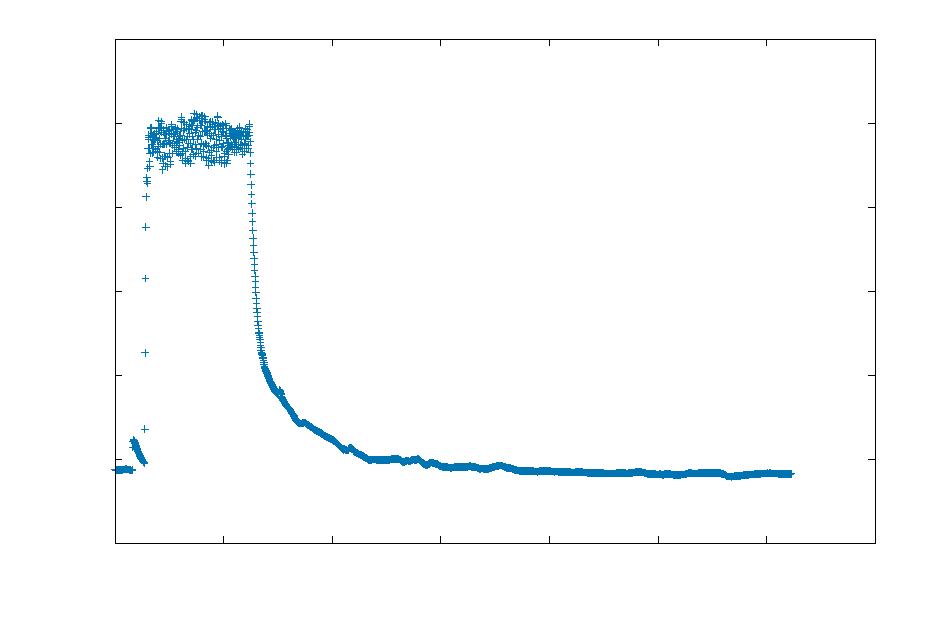
\includegraphics[width={432.00bp},height={288.00bp}]{relaxacni_doba_nezapouzdrene}}%
    \gplfronttext
  \end{picture}%
\endgroup

  \caption{relaxace}
\end{figure}

\begin{figure}[ht]
  \centering
  % GNUPLOT: LaTeX picture with Postscript
\begingroup
  \makeatletter
  \providecommand\color[2][]{%
    \GenericError{(gnuplot) \space\space\space\@spaces}{%
      Package color not loaded in conjunction with
      terminal option `colourtext'%
    }{See the gnuplot documentation for explanation.%
    }{Either use 'blacktext' in gnuplot or load the package
      color.sty in LaTeX.}%
    \renewcommand\color[2][]{}%
  }%
  \providecommand\includegraphics[2][]{%
    \GenericError{(gnuplot) \space\space\space\@spaces}{%
      Package graphicx or graphics not loaded%
    }{See the gnuplot documentation for explanation.%
    }{The gnuplot epslatex terminal needs graphicx.sty or graphics.sty.}%
    \renewcommand\includegraphics[2][]{}%
  }%
  \providecommand\rotatebox[2]{#2}%
  \@ifundefined{ifGPcolor}{%
    \newif\ifGPcolor
    \GPcolorfalse
  }{}%
  \@ifundefined{ifGPblacktext}{%
    \newif\ifGPblacktext
    \GPblacktexttrue
  }{}%
  % define a \g@addto@macro without @ in the name:
  \let\gplgaddtomacro\g@addto@macro
  % define empty templates for all commands taking text:
  \gdef\gplbacktext{}%
  \gdef\gplfronttext{}%
  \makeatother
  \ifGPblacktext
    % no textcolor at all
    \def\colorrgb#1{}%
    \def\colorgray#1{}%
  \else
    % gray or color?
    \ifGPcolor
      \def\colorrgb#1{\color[rgb]{#1}}%
      \def\colorgray#1{\color[gray]{#1}}%
      \expandafter\def\csname LTw\endcsname{\color{white}}%
      \expandafter\def\csname LTb\endcsname{\color{black}}%
      \expandafter\def\csname LTa\endcsname{\color{black}}%
      \expandafter\def\csname LT0\endcsname{\color[rgb]{1,0,0}}%
      \expandafter\def\csname LT1\endcsname{\color[rgb]{0,1,0}}%
      \expandafter\def\csname LT2\endcsname{\color[rgb]{0,0,1}}%
      \expandafter\def\csname LT3\endcsname{\color[rgb]{1,0,1}}%
      \expandafter\def\csname LT4\endcsname{\color[rgb]{0,1,1}}%
      \expandafter\def\csname LT5\endcsname{\color[rgb]{1,1,0}}%
      \expandafter\def\csname LT6\endcsname{\color[rgb]{0,0,0}}%
      \expandafter\def\csname LT7\endcsname{\color[rgb]{1,0.3,0}}%
      \expandafter\def\csname LT8\endcsname{\color[rgb]{0.5,0.5,0.5}}%
    \else
      % gray
      \def\colorrgb#1{\color{black}}%
      \def\colorgray#1{\color[gray]{#1}}%
      \expandafter\def\csname LTw\endcsname{\color{white}}%
      \expandafter\def\csname LTb\endcsname{\color{black}}%
      \expandafter\def\csname LTa\endcsname{\color{black}}%
      \expandafter\def\csname LT0\endcsname{\color{black}}%
      \expandafter\def\csname LT1\endcsname{\color{black}}%
      \expandafter\def\csname LT2\endcsname{\color{black}}%
      \expandafter\def\csname LT3\endcsname{\color{black}}%
      \expandafter\def\csname LT4\endcsname{\color{black}}%
      \expandafter\def\csname LT5\endcsname{\color{black}}%
      \expandafter\def\csname LT6\endcsname{\color{black}}%
      \expandafter\def\csname LT7\endcsname{\color{black}}%
      \expandafter\def\csname LT8\endcsname{\color{black}}%
    \fi
  \fi
    \setlength{\unitlength}{0.0500bp}%
    \ifx\gptboxheight\undefined%
      \newlength{\gptboxheight}%
      \newlength{\gptboxwidth}%
      \newsavebox{\gptboxtext}%
    \fi%
    \setlength{\fboxrule}{0.5pt}%
    \setlength{\fboxsep}{1pt}%
    \definecolor{tbcol}{rgb}{1,1,1}%
\begin{picture}(8640.00,5760.00)%
    \gplgaddtomacro\gplbacktext{%
      \csname LTb\endcsname%%
      \put(946,704){\makebox(0,0)[r]{\strut{}$1090$}}%
      \put(946,1144){\makebox(0,0)[r]{\strut{}$1100$}}%
      \put(946,1583){\makebox(0,0)[r]{\strut{}$1110$}}%
      \put(946,2023){\makebox(0,0)[r]{\strut{}$1120$}}%
      \put(946,2462){\makebox(0,0)[r]{\strut{}$1130$}}%
      \put(946,2902){\makebox(0,0)[r]{\strut{}$1140$}}%
      \put(946,3341){\makebox(0,0)[r]{\strut{}$1150$}}%
      \put(946,3781){\makebox(0,0)[r]{\strut{}$1160$}}%
      \put(946,4220){\makebox(0,0)[r]{\strut{}$1170$}}%
      \put(946,4660){\makebox(0,0)[r]{\strut{}$1180$}}%
      \put(946,5099){\makebox(0,0)[r]{\strut{}$1190$}}%
      \put(946,5539){\makebox(0,0)[r]{\strut{}$1200$}}%
      \put(1078,484){\makebox(0,0){\strut{}$0$}}%
      \put(2102,484){\makebox(0,0){\strut{}$200$}}%
      \put(3125,484){\makebox(0,0){\strut{}$400$}}%
      \put(4149,484){\makebox(0,0){\strut{}$600$}}%
      \put(5172,484){\makebox(0,0){\strut{}$800$}}%
      \put(6196,484){\makebox(0,0){\strut{}$1000$}}%
      \put(7219,484){\makebox(0,0){\strut{}$1200$}}%
      \put(8243,484){\makebox(0,0){\strut{}$1400$}}%
    }%
    \gplgaddtomacro\gplfronttext{%
      \csname LTb\endcsname%%
      \put(209,3121){\rotatebox{-270.00}{\makebox(0,0){\strut{}Odpor [$\Omega$]}}}%
      \put(4660,154){\makebox(0,0){\strut{}Čas [s]}}%
    }%
    \gplbacktext
    \put(0,0){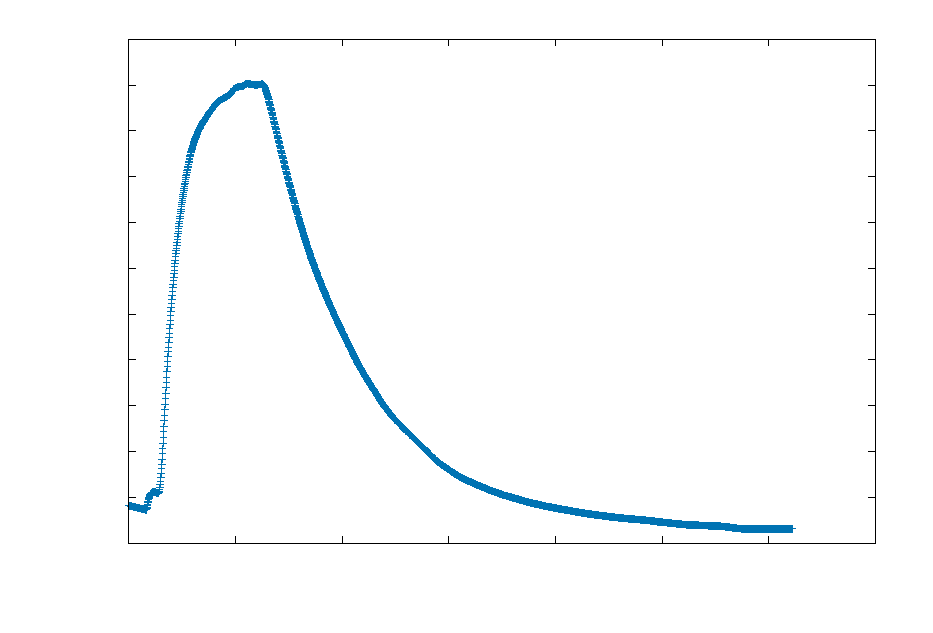
\includegraphics[width={432.00bp},height={288.00bp}]{relaxacni_doba_zapozdrene}}%
    \gplfronttext
  \end{picture}%
\endgroup

  \caption{}
\end{figure}

\subsection{Měření můstkem}

\begin{figure}[ht]
  \centering
  % GNUPLOT: LaTeX picture with Postscript
\begingroup
  \makeatletter
  \providecommand\color[2][]{%
    \GenericError{(gnuplot) \space\space\space\@spaces}{%
      Package color not loaded in conjunction with
      terminal option `colourtext'%
    }{See the gnuplot documentation for explanation.%
    }{Either use 'blacktext' in gnuplot or load the package
      color.sty in LaTeX.}%
    \renewcommand\color[2][]{}%
  }%
  \providecommand\includegraphics[2][]{%
    \GenericError{(gnuplot) \space\space\space\@spaces}{%
      Package graphicx or graphics not loaded%
    }{See the gnuplot documentation for explanation.%
    }{The gnuplot epslatex terminal needs graphicx.sty or graphics.sty.}%
    \renewcommand\includegraphics[2][]{}%
  }%
  \providecommand\rotatebox[2]{#2}%
  \@ifundefined{ifGPcolor}{%
    \newif\ifGPcolor
    \GPcolorfalse
  }{}%
  \@ifundefined{ifGPblacktext}{%
    \newif\ifGPblacktext
    \GPblacktexttrue
  }{}%
  % define a \g@addto@macro without @ in the name:
  \let\gplgaddtomacro\g@addto@macro
  % define empty templates for all commands taking text:
  \gdef\gplbacktext{}%
  \gdef\gplfronttext{}%
  \makeatother
  \ifGPblacktext
    % no textcolor at all
    \def\colorrgb#1{}%
    \def\colorgray#1{}%
  \else
    % gray or color?
    \ifGPcolor
      \def\colorrgb#1{\color[rgb]{#1}}%
      \def\colorgray#1{\color[gray]{#1}}%
      \expandafter\def\csname LTw\endcsname{\color{white}}%
      \expandafter\def\csname LTb\endcsname{\color{black}}%
      \expandafter\def\csname LTa\endcsname{\color{black}}%
      \expandafter\def\csname LT0\endcsname{\color[rgb]{1,0,0}}%
      \expandafter\def\csname LT1\endcsname{\color[rgb]{0,1,0}}%
      \expandafter\def\csname LT2\endcsname{\color[rgb]{0,0,1}}%
      \expandafter\def\csname LT3\endcsname{\color[rgb]{1,0,1}}%
      \expandafter\def\csname LT4\endcsname{\color[rgb]{0,1,1}}%
      \expandafter\def\csname LT5\endcsname{\color[rgb]{1,1,0}}%
      \expandafter\def\csname LT6\endcsname{\color[rgb]{0,0,0}}%
      \expandafter\def\csname LT7\endcsname{\color[rgb]{1,0.3,0}}%
      \expandafter\def\csname LT8\endcsname{\color[rgb]{0.5,0.5,0.5}}%
    \else
      % gray
      \def\colorrgb#1{\color{black}}%
      \def\colorgray#1{\color[gray]{#1}}%
      \expandafter\def\csname LTw\endcsname{\color{white}}%
      \expandafter\def\csname LTb\endcsname{\color{black}}%
      \expandafter\def\csname LTa\endcsname{\color{black}}%
      \expandafter\def\csname LT0\endcsname{\color{black}}%
      \expandafter\def\csname LT1\endcsname{\color{black}}%
      \expandafter\def\csname LT2\endcsname{\color{black}}%
      \expandafter\def\csname LT3\endcsname{\color{black}}%
      \expandafter\def\csname LT4\endcsname{\color{black}}%
      \expandafter\def\csname LT5\endcsname{\color{black}}%
      \expandafter\def\csname LT6\endcsname{\color{black}}%
      \expandafter\def\csname LT7\endcsname{\color{black}}%
      \expandafter\def\csname LT8\endcsname{\color{black}}%
    \fi
  \fi
    \setlength{\unitlength}{0.0500bp}%
    \ifx\gptboxheight\undefined%
      \newlength{\gptboxheight}%
      \newlength{\gptboxwidth}%
      \newsavebox{\gptboxtext}%
    \fi%
    \setlength{\fboxrule}{0.5pt}%
    \setlength{\fboxsep}{1pt}%
    \definecolor{tbcol}{rgb}{1,1,1}%
\begin{picture}(8640.00,3888.00)%
    \gplgaddtomacro\gplbacktext{%
      \csname LTb\endcsname%%
      \put(946,116){\makebox(0,0)[r]{\strut{}$-0.4$}}%
      \put(946,623){\makebox(0,0)[r]{\strut{}$-0.3$}}%
      \put(946,1131){\makebox(0,0)[r]{\strut{}$-0.2$}}%
      \put(946,1638){\makebox(0,0)[r]{\strut{}$-0.1$}}%
      \put(946,2145){\makebox(0,0)[r]{\strut{}$0$}}%
      \put(946,2652){\makebox(0,0)[r]{\strut{}$0.1$}}%
      \put(946,3160){\makebox(0,0)[r]{\strut{}$0.2$}}%
      \put(946,3667){\makebox(0,0)[r]{\strut{}$0.3$}}%
      \put(1078,-104){\makebox(0,0){\strut{}$0$}}%
      \put(1974,-104){\makebox(0,0){\strut{}$100$}}%
      \put(2869,-104){\makebox(0,0){\strut{}$200$}}%
      \put(3765,-104){\makebox(0,0){\strut{}$300$}}%
      \put(4661,-104){\makebox(0,0){\strut{}$400$}}%
      \put(5556,-104){\makebox(0,0){\strut{}$500$}}%
      \put(6452,-104){\makebox(0,0){\strut{}$600$}}%
      \put(7347,-104){\makebox(0,0){\strut{}$700$}}%
      \put(8243,-104){\makebox(0,0){\strut{}$800$}}%
    }%
    \gplgaddtomacro\gplfronttext{%
      \csname LTb\endcsname%%
      \put(209,1891){\rotatebox{-270.00}{\makebox(0,0){\strut{}$\Delta$t [$^{\circ} C$]}}}%
      \put(4660,-434){\makebox(0,0){\strut{}čas [s]}}%
    }%
    \gplbacktext
    \put(0,0){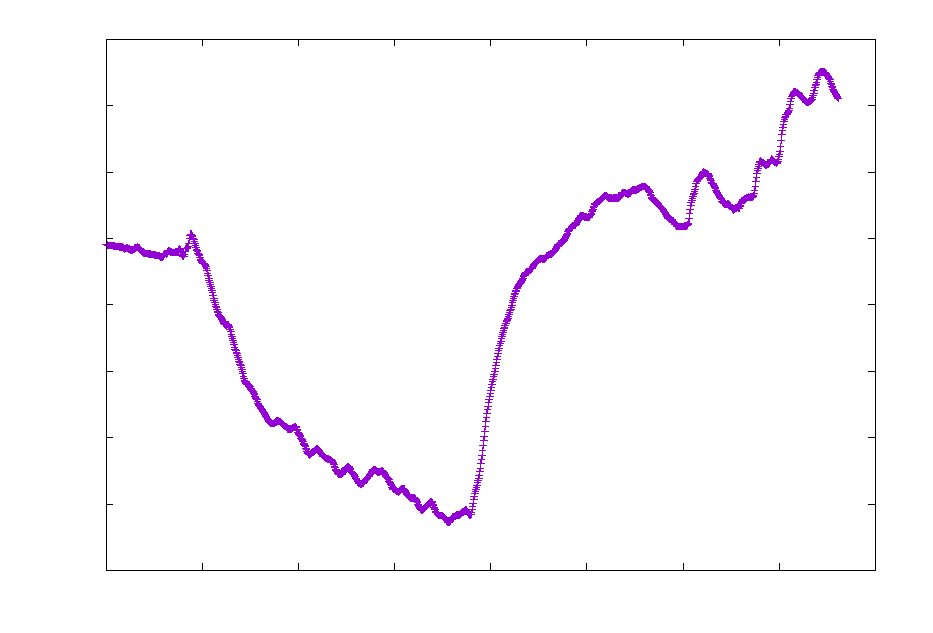
\includegraphics[width={432.00bp},height={194.40bp}]{mustek}}%
    \gplfronttext
  \end{picture}%
\endgroup

\end{figure}

\section{Závěr}

\begin{thebibliography}{0}
\bibitem{navody} Bochníček a kol. \textit{Fyzikální praktikum 1, návody k ulohám.} Brno 2024.\\ Dostupné z~\url{https://monoceros.physics.muni.cz/kof/vyuka/fp1_skripta.pdf}.   
\bibitem{tabulky} Hustota pevných látek. Dostupné z~\url{http://www.converter.cz/tabulky/hustota-pevne.htmf}.   
\end{thebibliography}

\end{document}
